\documentclass{beamer}
\usetheme{Copenhagen}
\usecolortheme{whale}
\usepackage{graphicx}
\usepackage{url}
\usepackage{amsmath}
\usepackage{tikz}
\usetikzlibrary{arrows.meta, positioning, calc}

\title{Stereo Vision}
\author[Fedya Semenov]{
  Fedya Semenov \\ 
  \vspace{0.3em}
  {\normalsize Advisors: Bill Breslin and Ian Besse}
}
\institute{Pacific University}
\date{October 26, 2026}

\begin{document}

\frame{\titlepage}

\begin{frame}
\frametitle{Outline}
\tableofcontents
\end{frame}

\section{Motivation}

\begin{frame}
\frametitle{Seeing Things Differently}
\begin{itemize}
    \item Depth perception: important \pause
    \item Needed by robots, drones, self-driving cars \pause
    \item LiDAR:
    \begin{itemize}
        \item Good, but expensive and bulky
        \item Can miss finer details and small objects
        \item Can malfunction in fog or rain
    \end{itemize} \pause
    \item Humans: good at perceiving depth \pause
    \item Why can't a machine perceive depth the same way a human does?
\end{itemize}
\end{frame}

\begin{frame}
\frametitle{Stereo Vision}
\begin{itemize}
    \item Why two eyes? \pause
    \item One eye closed $\rightarrow$ harder to perceive depth \pause
    \item Two eyes $\rightarrow$ easy depth perception, math behind it \pause
    \item For machines: two images from identical cameras placed a short distance apart to perceive depth \cite{scharstein2002taxonomy, zbontar2016stereo}
\end{itemize}
\end{frame}

\section{Stereo Geometry \& Disparity}

\begin{frame}
\frametitle{Stereo Vision Geometry}
\begin{itemize}
    \item Two cameras separated by baseline $B$ with focal length $f$
    \item 3D point $P$ projected onto left and right image planes
\end{itemize}
\centering
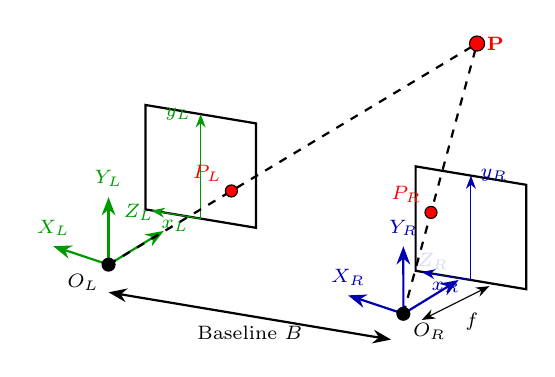
\begin{tikzpicture}[scale=0.78, every node/.style={font=\scriptsize}]
    % Left Camera Center
    \coordinate (OL) at (0,0);
    % Right Camera Center
    \coordinate (OR) at (4.8,-0.8);
    % 3D Point P
    \coordinate (P) at (6.0,3.6);

    % Left axes
    \draw[-Stealth, green!60!black, thick] (OL) -- (-0.9,0.3) node[above] {$X_L$};
    \draw[-Stealth, green!60!black, thick] (OL) -- (0,1.1) node[above] {$Y_L$};
    \draw[-Stealth, green!60!black, thick] (OL) -- (0.9,0.55) node[above left] {$Z_L$};

    % Right axes
    \draw[-Stealth, blue!70!black, thick] (OR) -- (3.9,-0.5) node[above] {$X_R$};
    \draw[-Stealth, blue!70!black, thick] (OR) -- (4.8,0.3) node[above] {$Y_R$};
    \draw[-Stealth, blue!70!black, thick] (OR) -- (5.7,-0.25) node[above left] {$Z_R$};

    % Left Image Plane
    \filldraw[fill=white, draw=black, thick, fill opacity=0.85]
        (0.6,0.9) -- (2.4,0.6) -- (2.4,2.3) -- (0.6,2.6) -- cycle;
    \draw[-Stealth, green!60!black] (1.5,0.75) -- (0.7,0.88) node[below right] {$x_L$};
    \draw[-Stealth, green!60!black] (1.5,0.75) -- (1.5,2.45) node[left] {$y_L$};

    % Right Image Plane
    \filldraw[fill=white, draw=black, thick, fill opacity=0.85]
        (5.0,-0.1) -- (6.8,-0.4) -- (6.8,1.3) -- (5.0,1.6) -- cycle;
    \draw[-Stealth, blue!70!black] (5.9,-0.25) -- (5.1,-0.12) node[below right] {$x_R$};
    \draw[-Stealth, blue!70!black] (5.9,-0.25) -- (5.9,1.45) node[right] {$y_R$};

    % Projection rays
    \draw[dashed, thick] (OL) -- (P);
    \draw[dashed, thick] (OR) -- (P);

    % Image projections
    \filldraw[red, draw=black] (2.0,1.2) circle (2.8pt) node[above left] {$P_L$};
    \filldraw[red, draw=black] (5.25,0.85) circle (2.8pt) node[above left] {$P_R$};

    % Camera centers and 3D Point
    \filldraw[black] (OL) circle (3pt) node[below left] {$O_L$};
    \filldraw[black] (OR) circle (3pt) node[below right] {$O_R$};
    \filldraw[red, draw=black] (P) circle (3.5pt) node[right] {$\mathbf{P}$};

    % Baseline B
    \draw[<->, >=Stealth, thick] (0,-0.45) -- (4.6,-1.22) node[midway, below] {Baseline $B$};

    % Focal length f
    \draw[<->, >=Stealth, thin] (5.1,-0.9) -- (6.2,-0.35) node[midway, below right] {$f$};
\end{tikzpicture}
\vspace{2pt}
{\tiny Diagram generated by Gemini \cite{gemini2026}}
\end{frame}

\begin{frame}
\frametitle{Epipolar Plane \& Epipolar Lines}
\begin{itemize}
    \item Epipolar plane: goes through both camera centers ($O_L, O_R$) and point $P$ in space
    \item Image projections: $P_L$ and $P_R$ on each camera plane
    \item Epipolar line: intersection of epipolar plane with image plane
\end{itemize}
\centering
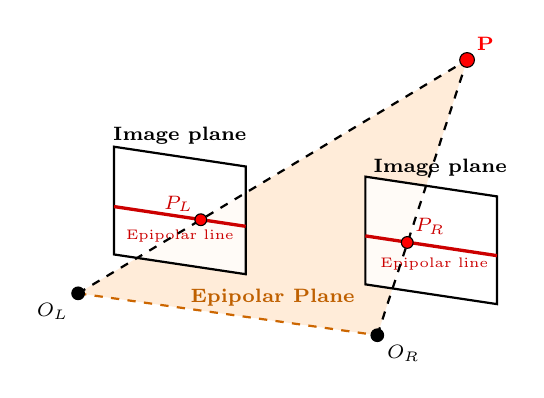
\begin{tikzpicture}[scale=0.76, every node/.style={font=\scriptsize}]
    % Camera centers and 3D point P
    \coordinate (OL) at (0,0);
    \coordinate (OR) at (5.0,-0.7);
    \coordinate (P)  at (6.5,3.9);

    % Epipolar Plane (shaded triangle)
    \fill[orange!20, fill opacity=0.75] (OL) -- (OR) -- (P) -- cycle;
    \draw[orange!80!black, dashed, thick] (OL) -- (OR);

    % Left Image Plane (x from 0.6 to 2.8)
    \filldraw[fill=white, draw=black, thick, fill opacity=0.82]
        (0.6,0.65) -- (2.8,0.32) -- (2.8,2.12) -- (0.6,2.45) -- cycle;
    \node[above, font=\scriptsize\bfseries] at (1.7,2.32) {Image plane};

    % Right Image Plane (x from 4.8 to 7.0)
    \filldraw[fill=white, draw=black, thick, fill opacity=0.82]
        (4.8,0.15) -- (7.0,-0.18) -- (7.0,1.62) -- (4.8,1.95) -- cycle;
    \node[above, font=\scriptsize\bfseries] at (6.05,1.80) {Image plane};

    % Epipolar Plane label shifted below the image planes
    \node[orange!75!black, font=\scriptsize\bfseries] at (3.25,-0.08) {Epipolar Plane};

    % Epipolar lines on planes (smaller font)
    \draw[red!80!black, very thick] (0.6,1.45) -- (2.8,1.12);
    \node[red!80!black, font=\tiny, below] at (1.70,1.22) {Epipolar line};

    \draw[red!80!black, very thick] (4.8,0.96) -- (7.0,0.63);
    \node[red!80!black, font=\tiny, below] at (5.95,0.75) {Epipolar line};

    % Projection rays from camera centers to P
    \draw[dashed, thick] (OL) -- (P);
    \draw[dashed, thick] (OR) -- (P);

    % Projections PL and PR (placed well inside the planes)
    \filldraw[red, draw=black] (2.05,1.23) circle (2.8pt);
    \node[red!80!black, font=\scriptsize\bfseries, above left, inner sep=2pt] at (2.02,1.26) {$P_L$};

    \filldraw[red, draw=black] (5.50,0.85) circle (2.8pt);
    \node[red!80!black, font=\scriptsize\bfseries, above right, inner sep=2pt] at (5.53,0.88) {$P_R$};

    % Centers & Point P
    \filldraw[black] (OL) circle (3pt) node[below left] {$O_L$};
    \filldraw[black] (OR) circle (3pt) node[below right] {$O_R$};
    \filldraw[red, draw=black] (P) circle (3.5pt) node[above right] {$\mathbf{P}$};
\end{tikzpicture}

\vspace{1pt}
{\tiny Diagram generated by Gemini \cite{gemini2026}}
\end{frame}

\begin{frame}
\frametitle{Image Shift \& Disparity}
\begin{itemize}
    \item Same 3D point shifted between the two images
    \item Any point in left image $\rightarrow$ shifted left in right image
    \item Finger test: hold finger up and close one eye at a time
\end{itemize}
\vspace{6pt}
\centering
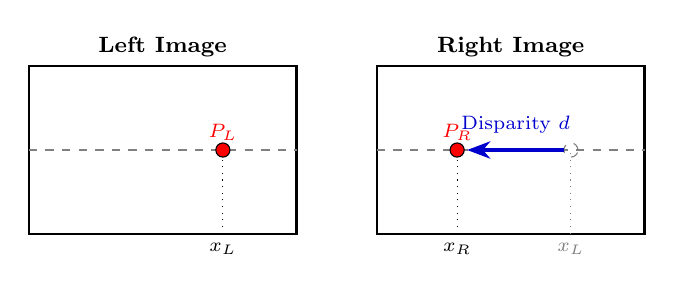
\begin{tikzpicture}[scale=0.85, every node/.style={font=\scriptsize}]
    % Left Image Box
    \draw[thick] (0,0) rectangle (4.0,2.5);
    \node[above, font=\footnotesize\bfseries] at (2.0,2.5) {Left Image};
    \draw[dashed, gray] (0,1.25) -- (4.0,1.25);
    \draw[dotted] (2.9,0) -- (2.9,1.25);
    \node[below] at (2.9,0) {$x_L$};
    \filldraw[red, draw=black] (2.9,1.25) circle (3pt) node[above] {$P_L$};

    % Right Image Box
    \draw[thick] (5.2,0) rectangle (9.2,2.5);
    \node[above, font=\footnotesize\bfseries] at (7.2,2.5) {Right Image};
    \draw[dashed, gray] (5.2,1.25) -- (9.2,1.25);

    % Ghost of Left position in Right image
    \draw[dotted, gray] (8.1,0) -- (8.1,1.25);
    \node[below, gray] at (8.1,0) {$x_L$};
    \draw[dashed, gray] (8.1,1.25) circle (3pt);

    % Shifted Right position
    \draw[dotted] (6.4,0) -- (6.4,1.25);
    \node[below] at (6.4,0) {$x_R$};
    \filldraw[red, draw=black] (6.4,1.25) circle (3pt) node[above] {$P_R$};

    % Disparity arrow
    \draw[-Stealth, blue!80!black, very thick] (8.0,1.25) -- (6.55,1.25)
        node[midway, above, yshift=2pt] {Disparity $d$};
\end{tikzpicture}
\vspace{2pt}
{\tiny Diagram generated by Gemini \cite{gemini2026}}
\end{frame}

\begin{frame}
\frametitle{The ``Disparity Trick''}
\begin{itemize}
    \item Disparity ($d$): shift between left and right image ($d = x_L - x_R$) \pause
    \item Points further out $\rightarrow$ smaller disparity \pause
    \item Verification: up-close finger shifts dramatically vs. distant object when closing/opening left and right eyes \pause
\end{itemize}
\begin{alertblock}{Depth Formula}
$$Z = \frac{B \cdot f}{d}$$
\end{alertblock}
\end{frame}

\begin{frame}
\frametitle{The ``Disparity Trick'': Geometry}
\begin{columns}[c,onlytextwidth]
    % Left Column: Similar Triangles Diagram
    \begin{column}{0.54\textwidth}
        \centering
        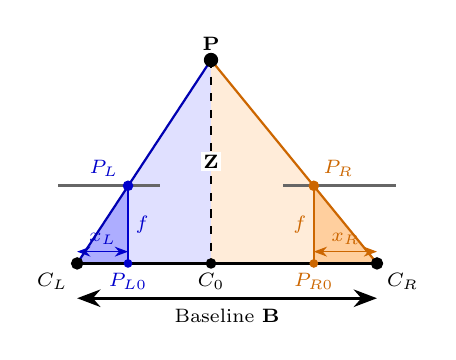
\begin{tikzpicture}[scale=0.68, every node/.style={font=\scriptsize}]
            % Coordinates
            \coordinate (CL)  at (0,0);
            \coordinate (CR)  at (5.6,0);
            \coordinate (P)   at (2.5,3.8);
            \coordinate (C0)  at (2.5,0);
            \coordinate (PL)  at (0.95,1.45);
            \coordinate (PL0) at (0.95,0);
            \coordinate (PR)  at (4.42,1.45);
            \coordinate (PR0) at (4.42,0);

            % Big Similar Triangles
            \fill[blue!12]   (CL) -- (P) -- (C0) -- cycle;
            \fill[orange!15] (CR) -- (P) -- (C0) -- cycle;

            % Small Similar Triangles (straight down to baseline)
            \fill[blue!32]   (CL) -- (PL) -- (PL0) -- cycle;
            \fill[orange!38] (CR) -- (PR) -- (PR0) -- cycle;

            % Image planes at height f = 1.45
            \draw[very thick, gray!80!black] (-0.35,1.45) -- (1.55,1.45);
            \draw[very thick, gray!80!black] (3.85,1.45) -- (5.95,1.45);

            % Vertical drops (straight down)
            \draw[thick, dashed] (P) -- (C0) node[midway, fill=white, inner sep=1pt] {$\mathbf{Z}$};
            \draw[thick, blue!80!black] (PL) -- (PL0) node[midway, right, xshift=-1pt] {$f$};
            \draw[thick, orange!80!black] (PR) -- (PR0) node[midway, left, xshift=1pt] {$f$};

            % Baseline segments
            \draw[thick] (CL) -- (CR);
            \draw[<->, >=Stealth, blue!80!black] (0,0.22) -- (0.95,0.22) node[midway, above, yshift=-1pt] {$x_L$};
            \draw[<->, >=Stealth, orange!80!black] (4.42,0.22) -- (5.6,0.22) node[midway, above, yshift=-1pt] {$x_R$};

            % Rays from cameras to P
            \draw[thick, blue!70!black] (CL) -- (P);
            \draw[thick, orange!80!black] (CR) -- (P);

            % Total Baseline B
            \draw[<->, >=Stealth, very thick] (0,-0.65) -- (5.6,-0.65) node[midway, below] {Baseline $\mathbf{B}$};

            % Points and Labels
            \filldraw[black] (CL)  circle (3pt) node[below left] {$C_L$};
            \filldraw[black] (CR)  circle (3pt) node[below right] {$C_R$};
            \filldraw[black] (C0)  circle (2.5pt) node[below] {$C_0$};
            \filldraw[blue!80!black] (PL0) circle (2pt) node[below] {$P_{L0}$};
            \filldraw[orange!80!black] (PR0) circle (2pt) node[below] {$P_{R0}$};
            \filldraw[blue!80!black] (PL)  circle (2.5pt) node[above left] {$P_L$};
            \filldraw[orange!80!black] (PR) circle (2.5pt) node[above right] {$P_R$};
            \filldraw[black] (P)   circle (3.5pt) node[above] {$\mathbf{P}$};
        \end{tikzpicture}
        \vspace{1pt}
        {\tiny Diagram generated by Gemini \cite{gemini2026}}
    \end{column}

    % Right Column: Variable Labels + Derivation
    \begin{column}{0.44\textwidth}
        \scriptsize
        \noindent
        $\mathbf{Z}$: Distance to $P$\\
        $\mathbf{B}$: Baseline distance\\
        $\mathbf{f}$: Focal length\\
        $\mathbf{d}$: Disparity ($x_L + x_R$)

        \vspace{-6pt}
        {\setlength{\jot}{1.5pt}
        \begin{align*}
            \frac{C_L \to C_0}{Z} &= \frac{x_L}{f} \\
            \frac{C_R \to C_0}{Z} &= \frac{x_R}{f} \\
            \frac{(C_L \to C_0) + (C_R \to C_0)}{Z} &= \frac{x_L + x_R}{f} \\
            \frac{B}{Z} &= \frac{d}{f} \\
            d &= \frac{B \cdot f}{Z} \\
            \mathbf{Z} &= \mathbf{\frac{B \cdot f}{d}}
        \end{align*}}
    \end{column}
\end{columns}
\end{frame}

\section{Rectification \& Matching}

\begin{frame}
\frametitle{Rectification}
\begin{itemize}
    \item Want horizontal epipolar lines on both images
    \item Needed due to:
    \begin{itemize}
        \item Camera tilt / misalignment
        \item Lenses distorting light
    \end{itemize}
    \item Goal: search along one horizontal line \cite{scharstein2002taxonomy}
\end{itemize}
\vspace{4pt}
\centering
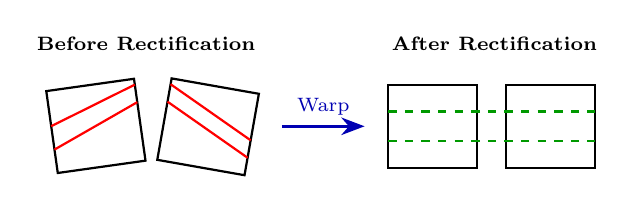
\begin{tikzpicture}[scale=0.75, every node/.style={font=\scriptsize}]
    % Unrectified pair
    \node[font=\scriptsize\bfseries] at (1.6,2.4) {Before Rectification};
    \begin{scope}[rotate around={8:(0.7,1.0)}]
        \draw[thick] (0,0.3) rectangle (1.5,1.7);
        \draw[red, thick] (0,0.7) -- (1.5,1.3);
        \draw[red, thick] (0,1.1) -- (1.5,1.6);
    \end{scope}
    \begin{scope}[rotate around={-10:(2.6,1.0)}]
        \draw[thick] (1.9,0.3) rectangle (3.4,1.7);
        \draw[red, thick] (1.9,1.3) -- (3.4,0.6);
        \draw[red, thick] (1.9,1.6) -- (3.4,0.9);
    \end{scope}

    % Warp Arrow
    \draw[-Stealth, very thick, blue!70!black] (3.9,1.0) -- (5.3,1.0)
        node[midway, above] {Warp};

    % Rectified pair
    \node[font=\scriptsize\bfseries] at (7.5,2.4) {After Rectification};
    \draw[thick] (5.7,0.3) rectangle (7.2,1.7);
    \draw[thick] (7.7,0.3) rectangle (9.2,1.7);
    \draw[green!60!black, thick, dashed] (5.7,0.75) -- (9.2,0.75);
    \draw[green!60!black, thick, dashed] (5.7,1.25) -- (9.2,1.25);
\end{tikzpicture}
\vspace{2pt}
{\tiny Diagram generated by Gemini \cite{gemini2026}}
\end{frame}

\begin{frame}
\frametitle{Finding Disparity}
\begin{itemize}
    \item Point in left image + where that point is in right image (disparity) $\rightarrow$ known depth \pause
    \item Core problem:
    \begin{itemize}
        \item Finding best disparity for each pixel \cite{scharstein2002taxonomy}
        \item Creating a dense depth map from a pair of stereo images \cite{scharstein2002taxonomy, zbontar2016stereo}
    \end{itemize}
\end{itemize}
\end{frame}

% --- PASTE STARTING HERE (Replaces the "TO BE CONTINUED" frame) ---

\begin{frame}
\frametitle{Simplest Algorithm}
\begin{itemize}
    \item Block-based search \cite{scharstein2002taxonomy} \pause
    \item For each pixel in left image $\rightarrow$ get block (window) of pixels around it \pause
    \item Start at same pixel in right image \pause
    \item Compare blocks $\rightarrow$ aggregated matching cost \pause
    \item Move window along scanline and repeat \pause
    \item Choose pixel with minimum aggregate matching cost as disparity value \pause
    \item Repeat on all pixels
\end{itemize}
\end{frame}

\begin{frame}
\frametitle{Simplest Algorithm: Block Shifting}
\centering
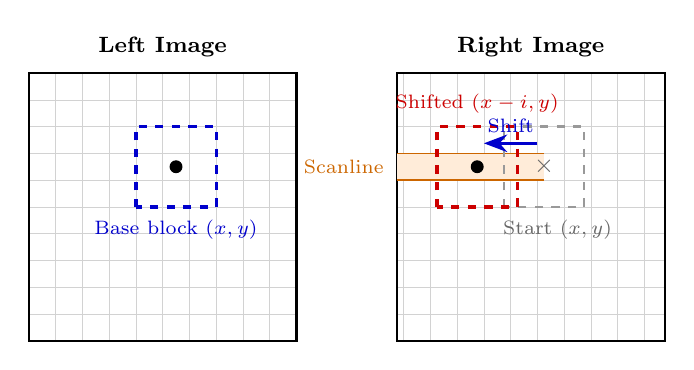
\begin{tikzpicture}[scale=0.85, every node/.style={font=\scriptsize}]
    % --- LEFT IMAGE ---
    \node[above, font=\footnotesize\bfseries] at (2.0, 4.1) {Left Image};
    % Pixel grid
    \draw[step=0.4, gray!35, very thin] (0,0) grid (4.0,4.0);
    \draw[thick] (0,0) rectangle (4.0,4.0);
    
    % Target pixel & dashed window around (2.2, 2.6)
    \draw[dashed, very thick, blue!80!black] (1.6,2.0) rectangle (2.8,3.2);
    \filldraw[black] (2.2,2.6) circle (2.5pt);
    \node[below, blue!80!black] at (2.2,1.95) {Base block $(x,y)$};

    % --- RIGHT IMAGE ---
    \node[above, font=\footnotesize\bfseries] at (7.5, 4.1) {Right Image};
    % Pixel grid
    \draw[step=0.4, gray!35, very thin] (5.5,0) grid (9.5,4.0);
    \draw[thick] (5.5,0) rectangle (9.5,4.0);

    % Horizontal scanline band going left from starting X
    \fill[orange!15] (5.5,2.4) rectangle (7.7,2.8);
    \draw[orange!80!black, semithick] (5.5,2.8) -- (7.7,2.8);
    \draw[orange!80!black, semithick] (5.5,2.4) -- (7.7,2.4);
    \node[left, orange!80!black] at (5.45,2.6) {Scanline};

    % Starting window at same (x,y) -> (7.7, 2.6) marked with X
    \draw[dashed, thick, gray!80] (7.1,2.0) rectangle (8.3,3.2);
    \node[font=\small\bfseries, gray!80!black] at (7.7,2.6) {$\times$};
    \node[below, gray!80!black] at (7.9,1.95) {Start $(x,y)$};

    % Shifted window at (x-i, y) -> (6.7, 2.6) marked with dot
    \draw[dashed, very thick, red!80!black] (6.1,2.0) rectangle (7.3,3.2);
    \filldraw[black] (6.7,2.6) circle (2.5pt);
    \node[above, red!80!black] at (6.7,3.25) {Shifted $(x-i, y)$};

    % Shift arrow
    \draw[-Stealth, very thick, blue!80!black] (7.6,2.95) -- (6.8,2.95)
        node[midway, above] {Shift};
\end{tikzpicture}
\vspace{2pt}
{\tiny Diagram generated by Gemini \cite{gemini2026}}
\end{frame}

\begin{frame}
\frametitle{Simplest Algorithm in Python (1/2)}
\centering
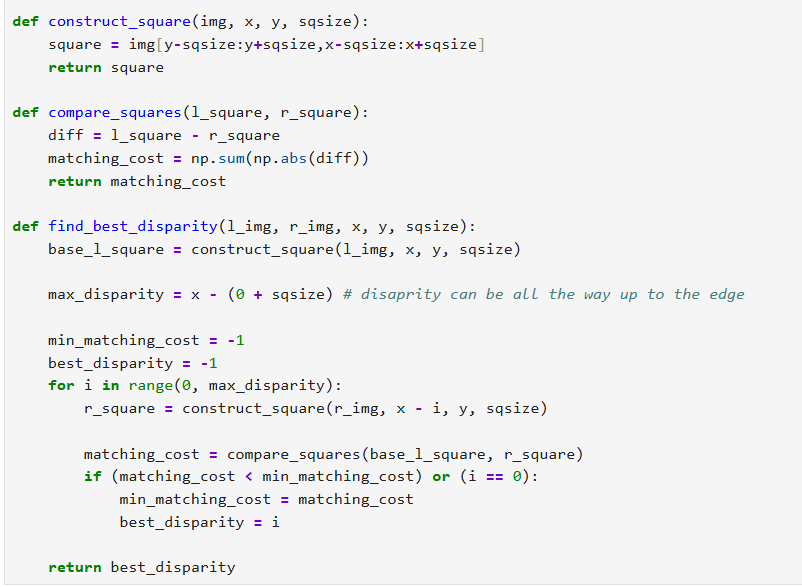
\includegraphics[width=0.95\textwidth, height=0.78\textheight, keepaspectratio]{SimpleAlgorithm1.png}
\end{frame}

\begin{frame}
\frametitle{Simplest Algorithm in Python (2/2)}
\centering
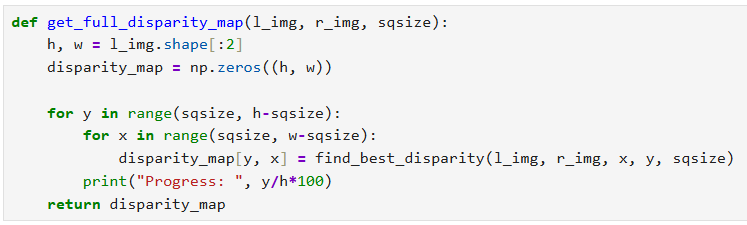
\includegraphics[width=0.95\textwidth, height=0.55\textheight, keepaspectratio]{SimpleAlgorithm2.png}
\vspace{8pt}
\begin{itemize}
    \item Good, clear implementation
    \item Really, really slow
\end{itemize}
\end{frame}

\begin{frame}
\frametitle{Testing on Some Images}
\centering
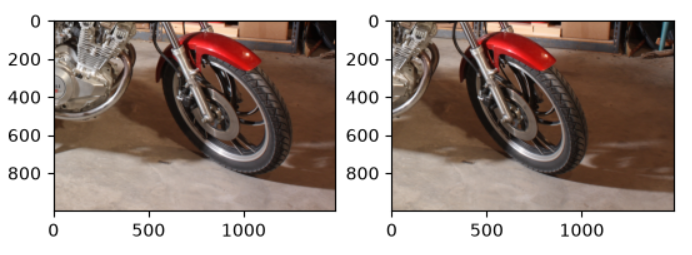
\includegraphics[width=0.92\textwidth, height=0.55\textheight, keepaspectratio]{LeftRightImages.png}
\vspace{6pt}
\begin{itemize}
    \item Images shifted
    \item $1000 \times 1200$ pixel images $\rightarrow$ took 1.5 hours
\end{itemize}
\end{frame}

\begin{frame}
\frametitle{Testing on Some Images: Result}
\centering
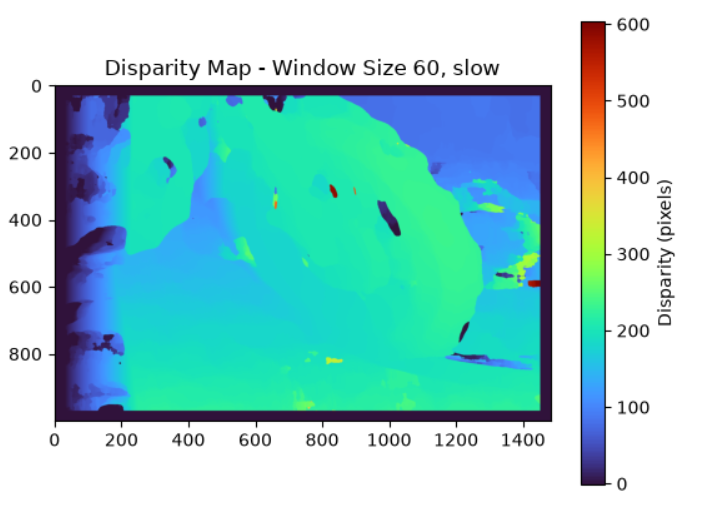
\includegraphics[width=0.88\textwidth, height=0.80\textheight, keepaspectratio]{DisparityResult1.png}
\end{frame}

\begin{frame}
\frametitle{Speeding Things Up}
\begin{itemize}
    \item Vectorize cost computation between pixels all at once
\end{itemize}
\centering
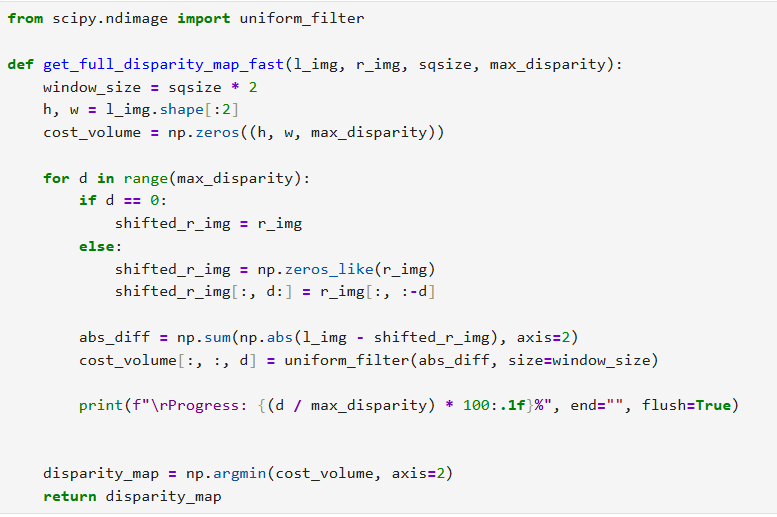
\includegraphics[width=0.95\textwidth, height=0.55\textheight, keepaspectratio]{FastSimpleAlgorithm.png}
\begin{itemize}
    \item Runs in about 1 minute
\end{itemize}
\end{frame}

\begin{frame}
\frametitle{Varying Window Size: Window Size 100}
\begin{itemize}
    \item Results vary greatly based on window size
    \item How big should comparison blocks be?
\end{itemize}
\centering
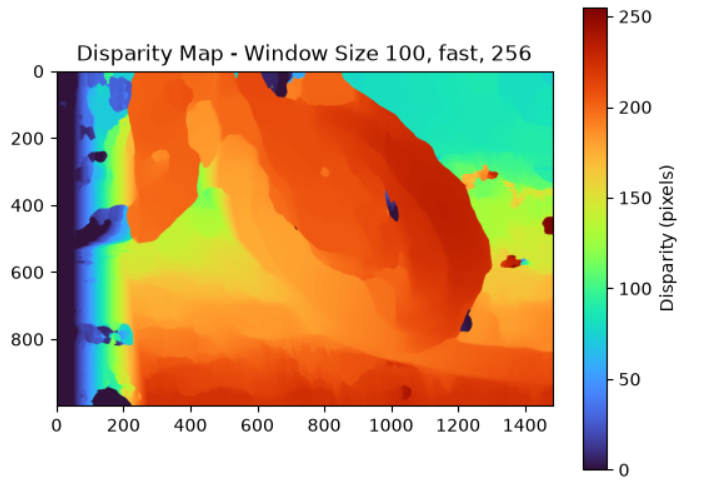
\includegraphics[width=0.82\textwidth, height=0.62\textheight, keepaspectratio]{DisparityResult2.png}
\end{frame}

\begin{frame}
\frametitle{Varying Window Size: Window Size 20}
\centering
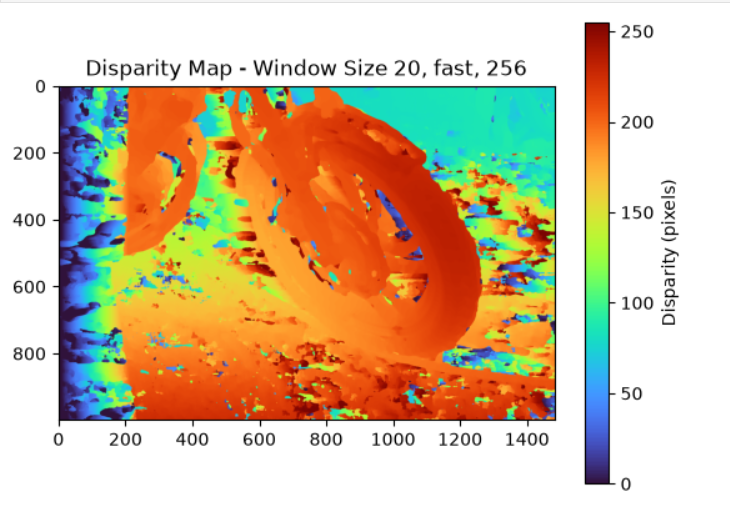
\includegraphics[width=0.88\textwidth, height=0.80\textheight, keepaspectratio]{DisparityResult3.png}
\end{frame}

\begin{frame}
\frametitle{Varying Window Size: Window Size 11}
\centering
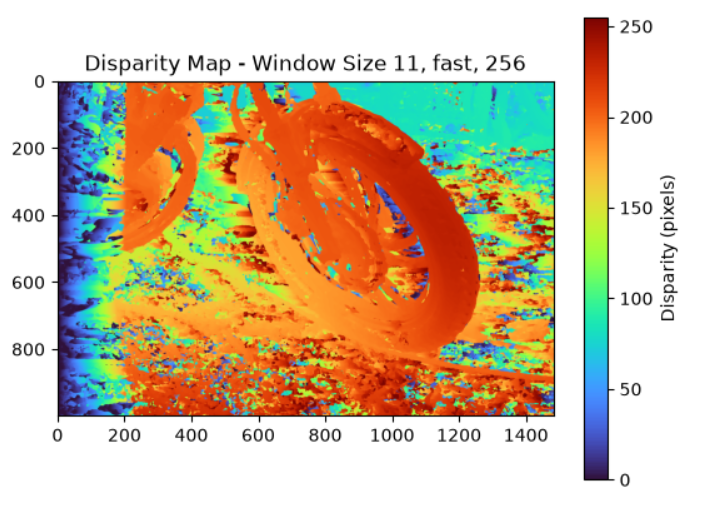
\includegraphics[width=0.88\textwidth, height=0.80\textheight, keepaspectratio]{DisparityResult4.png}
\end{frame}

\section{Advanced \& Deep Learning Approaches}

\begin{frame}
\frametitle{Beyond Block Matching}
\begin{itemize}
    \item Many improvements and better algorithms \cite{scharstein2002taxonomy}: \pause
    \begin{itemize}
        \item SGBM (Semi-Global Block Matching)
        \item Global Optimization
        \item Pre-Processing and Transforming Pixels
        \item Refinement Methods
    \end{itemize} \pause
    \item Good, can be fast
    \item Rely on human-designed procedure
\end{itemize}
\end{frame}

\begin{frame}
\frametitle{Deep Learning Algorithms}
\begin{itemize}
    \item Train on large sets of images with known ground truth depth maps \cite{zbontar2016stereo, HAMID20221663} \pause
    \item Pick up patterns and ``real world'' knowledge otherwise hard to detect \pause
    \item 2D algorithms: faster, don't compare disparity levels between pixels \cite{HAMID20221663} \pause
    \item 3D algorithms: slower, more depth awareness \cite{HAMID20221663} \pause
    \item Training data strongly influences performance:
    \begin{itemize}
        \item Different environment (e.g., indoors vs. outdoors) $\rightarrow$ worse performance \cite{HAMID20221663}
    \end{itemize}
\end{itemize}
\end{frame}

\begin{frame}
\frametitle{Project Goals}
\begin{itemize}
    \item Keep developing understanding of algorithms and tradeoffs: \pause
    \begin{itemize}
        \item Preferred environment, speed, accuracy, hardware requirements
    \end{itemize} \pause
    \item Try to train a model improving on one tradeoff: \pause
    \begin{itemize}
        \item Idea: Combine existing training datasets
        \item Idea: Add pre-processing step (object detection highlights?)
    \end{itemize}
\end{itemize}
\end{frame}

\section{References}
\begin{frame}{References}
\scriptsize
\nocite{*}
\bibliographystyle{amsplain}
\bibliography{references.bib}
\end{frame}

\end{document}